\documentclass[
  % all of the below options are optional and can be left out
  % course name (default: 2IL50 Data Structures)
  course = {{16-811 Math Fundamentals for Robotics}},
  % quartile (default: 3)
  quartile = {{1}},
  % assignment number/name (default: 1)
  assignment = 4,
  % student name (default: Some One)
  name = {{Kangle Deng}},
  % student number, NOT S-number (default: 0123456)
  % studentnumber = {{0123456 ; 0314159}},
  % student email (default: s.one@student.tue.nl)
  email = {{kangled@andrew.cmu.edu}},
  % first exercise number (default: 1)
  firstexercise = 1
]{aga-homework}

\usepackage{subfigure}

\begin{document}

\exercise
\subexercise

\begin{equation*}
\begin{aligned}
& 3y^2y' = 1 \\
\Rightarrow \qquad & 3y^2\frac{dy}{dx} = 1\\
\Rightarrow \qquad & 3y^2 dy = dx \\
\Rightarrow \qquad & \int 3y^2 dy = \int dx \\
\Rightarrow \qquad & y^3 = x + c \\ 
\Rightarrow \qquad & y = (x + c)^\frac{1}{3}.
\end{aligned}
\end{equation*}

Since $y(1) = 1$, we have $c = 0$. So, $y(x) = x^\frac{1}{3}$.

\subexercise

I implement this as a function $EulerMethod$ in $ex1.py$. See Table \ref{tab:hw4_ex1} and Figure \ref{fig:hw4_ex1} for the results.

\subexercise

I implement this as a function $Runge\_Kutta\_4$ in $ex1.py$. See Table \ref{tab:hw4_ex1} and Figure \ref{fig:hw4_ex1} for the results.

\subexercise

I implement this as a function $Adams\_Bashforth\_4$ in $ex1.py$. See Table \ref{tab:hw4_ex1} and Figure \ref{fig:hw4_ex1} for the results.

\begin{table}[h]
  \begin{center}
  \scriptsize{
    \begin{tabular}{c|c|cc|cc|cc}
      \toprule
      & & \multicolumn{2}{c}{Euler Method} & \multicolumn{2}{c}{Runge-Kutta-4} & \multicolumn{2}{c}{Adams-Bashforth-4} \\
     $\mathbf{x_i}$ & $\mathbf{y(x_i)}$ & $\mathbf{y_i}$ & $\mathbf{|y(x_i) - y_i|}$ & $\mathbf{y_i}$ & $\mathbf{|y(x_i) - y_i|}$ & $\mathbf{y_i}$ & $\mathbf{|y(x_i) - y_i|}$ \\
      \midrule
    1 & 1 & 1 & 0 & 1 & 0 & 1 & 0\\
    0.95 & 0.98304757 & 0.98333333 & 2.85760842e-04 & 0.98304757 & 2.31545783e-10 & 0.98304789 & 3.13269674e-07\\
    0.9 & 0.96548938 & 0.96609691 & 6.07522413e-04 & 0.96548938 & 5.35422817e-10 & 0.96549012 & 7.31959019e-07\\
    0.85 & 0.94726824 & 0.94823995 & 9.71716395e-04 & 0.94726824 & 9.38114586e-10 & 0.9472695 & 1.26719122e-06\\
    0.8  & 0.92831777 & 0.92970411 & 1.38634783e-03 & 0.92831777 & 1.47800661e-09 & 0.92831974 & 1.97537738e-06\\
    0.75 & 0.9085603 & 0.9104218 & 1.86150001e-03 & 0.90856029 & 2.21192253e-09 & 0.90856322 & 2.92094417e-06\\
    0.7 &  0.887904 &  0.89031405 & 2.41004564e-03 & 0.887904 & 3.22601024e-09 & 0.8879082 & 4.20008978e-06\\
    0.65 & 0.86623911 &  0.86928777 & 3.04866908e-03 & 0.8662391 & 4.65446159e-09 & 0.86624506 & 5.95950646e-06\\
    0.6 & 0.84343267 &  0.84723204 & 3.79937051e-03 & 0.84343266 & 6.71290179e-09 & 0.84344109 & 8.42671210e-06 \\
    0.55 & 0.81932127 & 0.82401301 & 4.69173849e-03 & 0.81932126 & 9.76049064e-09 & 0.81933324 &  1.19659070e-05\\
    0.5 &  0.79370053 & 0.79946702  & 5.76648969e-03 & 0.79370051 & 1.44211745e-08 & 0.79371771 & 1.71814172e-05\\
    0.45  & 0.76630943 & 0.77339061 & 7.08118241e-03 & 0.76630941 & 2.18343528e-08 & 0.76633455 &  2.51188322e-05\\
    0.4 &  0.7368063 & 0.74552613 & 8.71983432e-03 & 0.73680627 & 3.42096184e-08 & 0.73684398 & 3.76794301e-05\\
    0.35 & 0.70472987  & 0.71553983 & 1.08099523e-02 & 0.70472982 & 5.61603901e-08 & 0.70478841 & 5.85345338e-05\\
    0.3 & 0.66943295 & 0.68298757 & 1.35546167e-02 & 0.66943285 & 9.82575634e-08 & 0.66952827 &  9.53188261e-05\\
    0.25 & 0.62996052 & 0.64725838 & 1.72978532e-02 & 0.62996034 & 1.87832257e-07 & 0.630126 &  1.65472719e-04 \\
    0.2 & 0.58480355 & 0.60747576 & 2.26722099e-02 & 0.58480314 & 4.08116652e-07 & 0.58511762 &  3.14069523e-04\\
    0.15 & 0.53132928 & 0.56231192 & 3.09826343e-02 & 0.5313282 & 1.07988141e-06 & 0.53200856 &  6.79277176e-04\\
    0.1 & 0.46415888 & 0.50960178 & 4.54428953e-02 & 0.46415489 & 3.99451355e-06 & 0.46596718 &  1.80829890e-03\\
    0.05 & 0.36840315 & 0.44542368 & 7.70205253e-02 & 0.36837441 & 2.87377838e-05 & 0.37550918 &  7.10603329e-03\\
    0  & 0 & 0.36141925 & 3.61419252e-01 &  0.10345536 &  1.03455365e-01 & 0.22081638 & 2.20816379e-01\\
      \bottomrule
    \end{tabular}
    }
  \end{center}
\caption{\textbf{Ex 1}} 
 \label{tab:hw4_ex1}
\end{table}

\begin{figure}
    \centering
    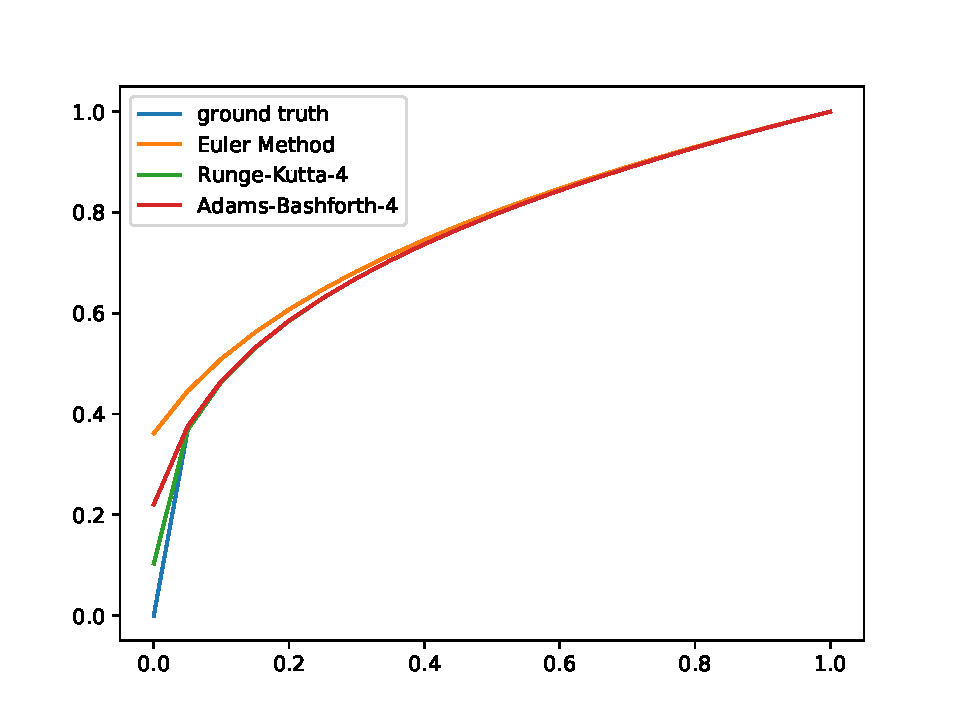
\includegraphics{math/fig/hw4/ex1.pdf}
    \caption{\textbf{Ex 1}}
    \label{fig:hw4_ex1}
\end{figure}

\exercise
\subexercise
The iso-contours are:
\begin{equation*}
    \begin{aligned}
    \frac{\partial f}{\partial x} = 3x^2 - 4x = 0 \Rightarrow x_1 = 0, \quad x_2 = \frac{4}{3}\\
    \frac{\partial f}{\partial y} = 3y^2 + 6y = 0 \Rightarrow y_1 = 0, \quad y_2 = -2
    \end{aligned}
\end{equation*}

So there are 4 critical points: $(0, 0), (0, -2), (\frac{4}{3}, 0), (\frac{4}{3}, -2)$.

Note that 

\begin{equation*}
    \frac{\partial f}{\partial x} 
    \begin{cases}
> 0, & x<0,\\
< 0,& 0 < x < \frac{4}{3},\\
> 0, & x > \frac{4}{3}.\\
\end{cases}
\end{equation*}

\begin{equation*}
    \frac{\partial f}{\partial y} 
    \begin{cases}
> 0, & y < -2,\\
< 0,& -2 < y < 0,\\
> 0, & y > 0.\\
\end{cases}
\end{equation*}

Therefore, $(0,-2)$ is local maxima, $(\frac{4}{3}, 0)$ is local minimum, $(0,0)$ and $(\frac{4}{3}, -2)$ are saddle points.

\subexercise
\noindent\textbf{1st step:} $(x_0, y_0) = (1, -1), (\frac{\partial f}{\partial x_0}, \frac{\partial f}{\partial y_0})= (-1, -3)$.

$f(x_0-\alpha \frac{\partial f}{\partial x_0}, y_0 - \alpha \frac{\partial f}{\partial y_0}) = f(1 + \alpha, -1 + 3\alpha) = g(\alpha).$

$0 = g'(\alpha) = 3(1+\alpha)^2 + 9(-1+3\alpha)^2 - 4(1+\alpha) + 18(-1+3\alpha) \Rightarrow (3\alpha - 1)(14 \alpha + 5) = 0.$

$\Rightarrow \alpha = \frac{1}{3}, (x_1, y_1) = (x_0, y_0) - \alpha (\frac{\partial f}{\partial x_0}, \frac{\partial f}{\partial y_0}) = (\frac{4}{3}, 0)$.

So only 1 step is needed to converge.

\exercise
\subexercise
Let $v_1, v_2$ be any 2 eigenvectors of $Q$, and $\lambda_1, \lambda_2$ be their eigenvalues ($\lambda_1 \ne \lambda_2$). Then we have:

\begin{equation*}
    \begin{aligned}
    Qv_1 = \lambda_1 v_1 \\
    Qv_2 = \lambda_2 v_2
    \end{aligned}
\end{equation*}

So,
\begin{equation*}
    \begin{aligned}
    v_2^TQv_1 = v_2^T(\lambda_1 v_1) = \lambda_1 v_2^T v_1 \\ 
    v_1^TQv_2 = v_1^T(\lambda_2 v_2) = \lambda_2 v_1^T v_2
    \end{aligned}
\end{equation*}

Note that $v_2^TQv_1 = (v_1^TQv_2)^T$ because $Q^T = Q$. So,

\begin{equation*}
\begin{aligned}
   & \lambda_1 v_2^T v_1 = (\lambda_2 v_1^T v_2)^T = \lambda_2 v_2^T v_1 \\
   \Rightarrow \qquad & (\lambda_1 - \lambda_2)  v_2^T v_1 = 0.
\end{aligned}

\end{equation*}

Since $\lambda_1 \ne \lambda_2$, we have $v_2^T v_1 = 0$. So $v_2^TQv_1 = v_1^TQv_2 = 0$.

\subexercise
Let $v_1, v_2$ be any 2 such orthogonal basis vector, and $\lambda_1, \lambda_2$ be their eigenvalues. Then $v_1^Tv_2 = 0$. So, 
\begin{equation*}
    v_1^TQv_2 = v_1^T(\lambda_2v_2) = \lambda v_1^Tv_2 = 0.
\end{equation*}

\exercise
\subexercise
Note that $d_{k} = -g_k + \beta_{k-1}d_{k-1} \Rightarrow d_k + g_k = \beta_{k-1}d_{k-1}$. So,

\begin{equation*}
    d_k^TQ(d_k + g_k) = d_k^TQ(\beta_{k-1}d_{k-1}) = \beta_{k-1} d_k^TQd_{k-1} = 0.
\end{equation*}
which is because all the $d_i$ are pair-wise $Q-$orthogonal.

Therefore, $d_k^TQd_k = -d_k^TQg_k$.

For each step of the conjugate gradient method, we should compute:
\begin{equation*}
    \begin{aligned}
       \alpha_k & = -\frac{g_k^Td_k}{d_k^TQd_k} = \frac{g_k^Td_k}{d_k^T(Qg_k)}, \\
       x_{k+1} & = x_k + \alpha_k d_k, \\
       \beta_k & = \frac{g_{k+1}^TQd_k}{d_k^TQd_k} = -\frac{(Qg_{k+1})^Td_k}{d_k^T(Qg_k)}, \\
       d_{k+1} & = -g_{k+1} + \beta_k d_k.
    \end{aligned}
\end{equation*}
So if we has already known $g_k$ and $Qg_k$, we don't need to use $Q$.

\subexercise
Note that
\begin{equation*}
    \begin{aligned}
       & g_k = Qx_k + b, \\
       & p_k = Qy_k + b.
    \end{aligned}
\end{equation*}
So, $g_k - p_k = Qx_k - Qy_k = Q(x_k - y_k) = Qg_k$.

\subexercise
% To avoid the knowledge of the Hessian $H$ of $f$ or a line search, we need to find a way to compute or approximate $\alpha_k$ that minimizes $f(x_k + \alpha_k d_k)$ for each step.

% From Taylor Expansion, we have:
% \begin{equation*}
% \begin{aligned}
%       f(x_k + \alpha d_k) \approx f(x_k) + \alpha_k (\nabla f(x_k))^T d_k + \frac{1}{2} \alpha_k^2 d_k^T H_f d_k. \\
%       0 = \frac{df(x_k + \alpha d_k)}{d\alpha} \approx (\nabla f(x_k))^T d_k + \alpha_k d_k^T H_f d_k \Rightarrow \alpha_k \approx -\frac{(\nabla f(x_k))^T d_k}{d_k^T H_f d_k}.
% \end{aligned}
% \end{equation*}
% So we only need to compute or approximate $H_f d_k$.

The algorithm is as follow:

\begin{algorithm}[H]
  \caption{Conjugate Gradient Method($f, x_0$)}
  \KwIn{A general function $f$ of which gradients $\nabla f$ can be computed, and a starting point $x_0$.}
  \KwOut{The local minimum of $f$.}

  $g_0 \leftarrow \nabla f(x_0)$ \;
  $d_0 \leftarrow -g_0$ \;
  \For{$k \leftarrow 0$ \To $n-1$}{
    $y_k \leftarrow x_k - g_k$ \;
    $p_k \leftarrow \nabla f(y_k)$ \;
    $t_k \leftarrow g_k - p_k$ \;
    $\alpha_k \leftarrow \frac{g_k^Td_k}{d_k^Tt_k}$ \;
    $x_{k+1} & = x_k + \alpha_k d_k$ \;
    $g_{k+1} = \nabla f(x_{k+1})$ \;
    $\beta_k = \frac{|\nabla f(x_{k+1})|^2}{|\nabla f(x_{k})|^2}$ \;
    $d_{k+1} & = -g_{k+1} + \beta_k d_k$ \;
  }

  \Return{$x_n, f(x_n)$}
\end{algorithm}

\exercise
We can formulate this as follow:

\begin{equation*}
    \max \limits_{x>0, y>0} xy \qquad \text{s.t. } x + y = p,
\end{equation*}
which is equivalent to:

\begin{equation*}
    \min \limits_{x>0, y>0} -xy \qquad \text{s.t. } x + y = p,
\end{equation*}

So we define Lagrange funtion as:

\begin{equation*}
    L(x,y,\lambda) = -xy + \lambda(x+y-p).
\end{equation*}

Then,
\begin{equation*}
\left\{
    \begin{aligned}
       \frac{\partial L}{\partial x} = -y + \lambda = 0,\\
       \frac{\partial L}{\partial y} = -x + \lambda = 0,\\
       \frac{\partial L}{\partial \lambda} = x + y -p =0.\\
    \end{aligned}
\right.
\end{equation*}

The solution is: $x = y = \lambda = \frac{p}{2}$. So the maximum area is $\frac{p^2}{4}$ when the perimeter of a rectangle is $2p$.

Below we will verify the the second-order sufficiency condition:
\begin{equation*}
    [\nabla^2 f] = \left(
    \begin{array}{cc}
        0 & -1 \\
        -1 & 0
    \end{array}
    \right).
\end{equation*}

\begin{equation*}
    [\nabla^2 h] = \left(
    \begin{array}{cc}
        0 & 0 \\
        0 & 0
    \end{array}
    \right).
\end{equation*}

So, $[\nabla^2 f] + \lambda [\nabla^2 h] = [\nabla^2 f] = \left(
    \begin{array}{cc}
        0 & -1 \\
        -1 & 0
    \end{array}
    \right)$.
On the other hand, the subspace perpendicular to $\nabla h$ is spanned by $\{(1,-1)^T\}$. Let $y$ be any vector in that space, so $y = (a, -a)^T$.

Then, $y^T([\nabla^2 f] + \lambda [\nabla^2 h])y = 2a^2$ is always greater than 0 when $y \ne 0$. So this solution satisfies the second-order sufficiency condition.

\exercise
\subexercise
I implement this in $ex6a.py$. I report the result after 100000 iterations as convergence result. See Figure \ref{fig:hw4_ex6a} for the results.

After 1 iteration, the path is moving away from the obstacles very little so we cannot clearly see it. After 30 iterations, we can clearly see the trend. In the convergence result, the path is broken into segments.

\begin{figure}
    \centering
    \subfigure[After 1 iter]{
    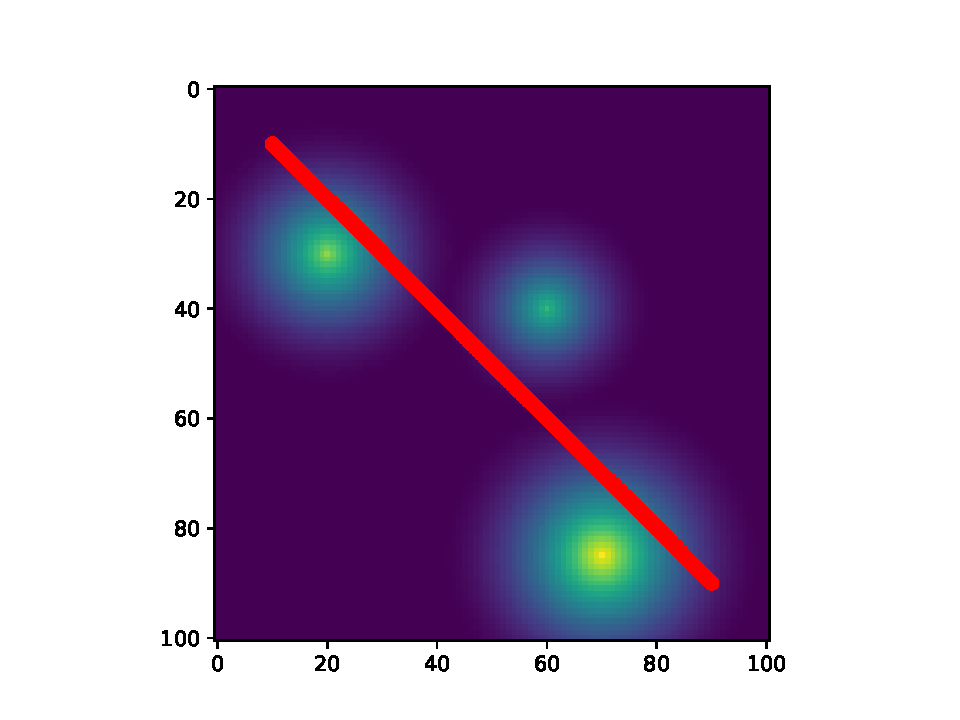
\includegraphics[width=.3\textwidth]{math/fig/hw4/ex6a/00000.pdf}
    }
    \subfigure[After 30 iters]{
    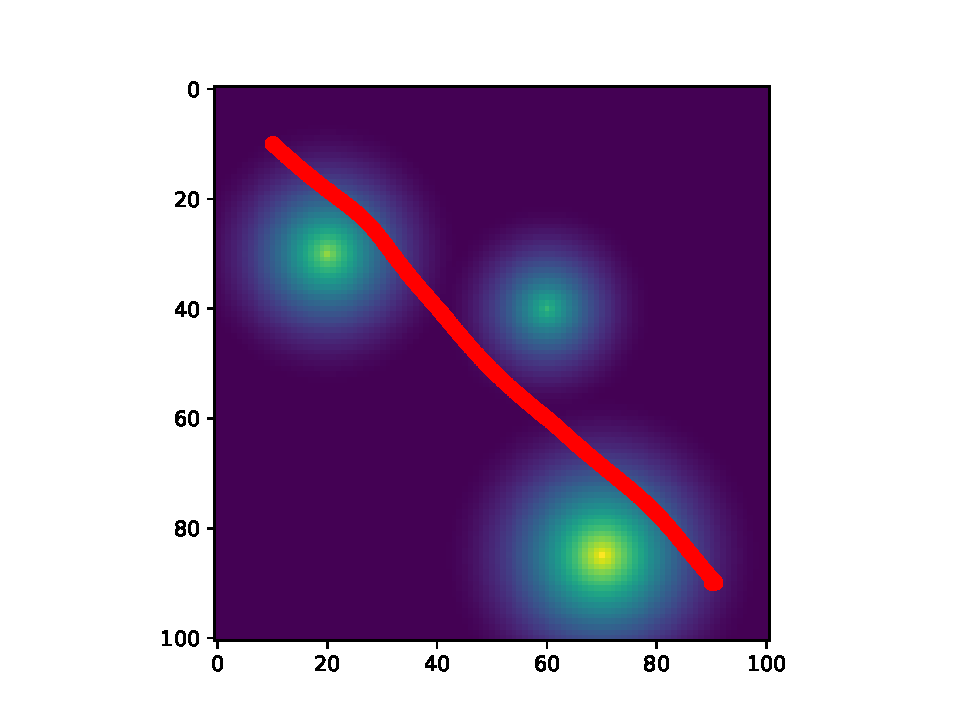
\includegraphics[width=.3\textwidth]{math/fig/hw4/ex6a/00030.pdf}
    }
    \subfigure[After 10000 iters (convergence)]{
    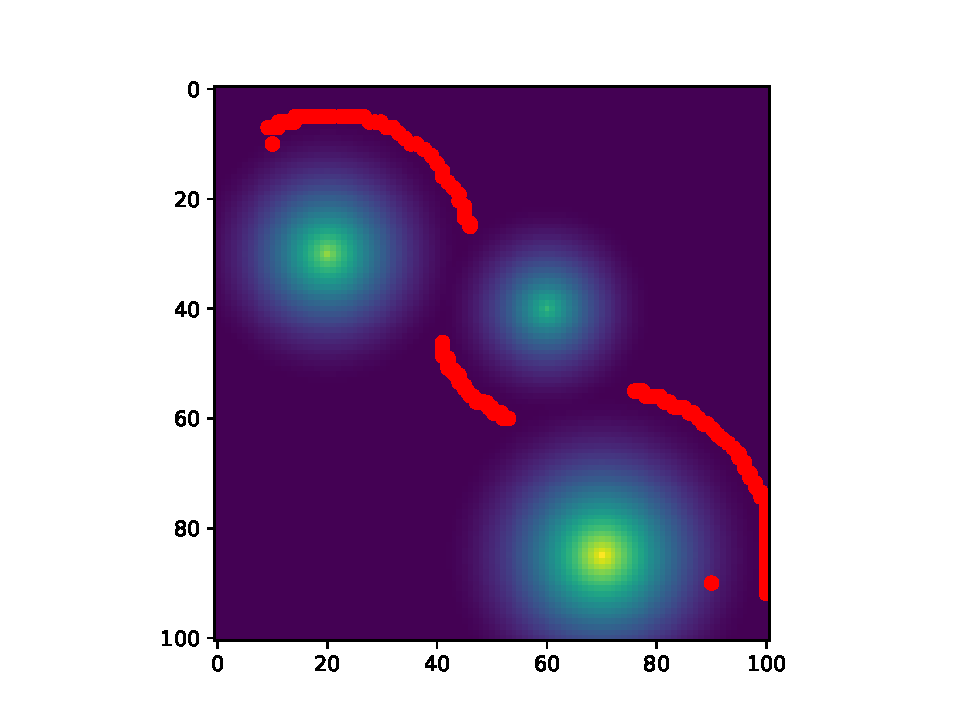
\includegraphics[width=.3\textwidth]{math/fig/hw4/ex6a/final.pdf}
    }
    \caption{\textbf{Ex 6a}}
    \label{fig:hw4_ex6a}
\end{figure}

\subexercise
Figure \ref{fig:hw4_ex6b} is the result. It does not work because it only considers the distance from the previous point in the path, but the last endpoint is fixed. So there is no restrictions that make the point prior to the last endpoint close to it.

\begin{figure}
    \centering
    \subfigure[After 100 iters]{
    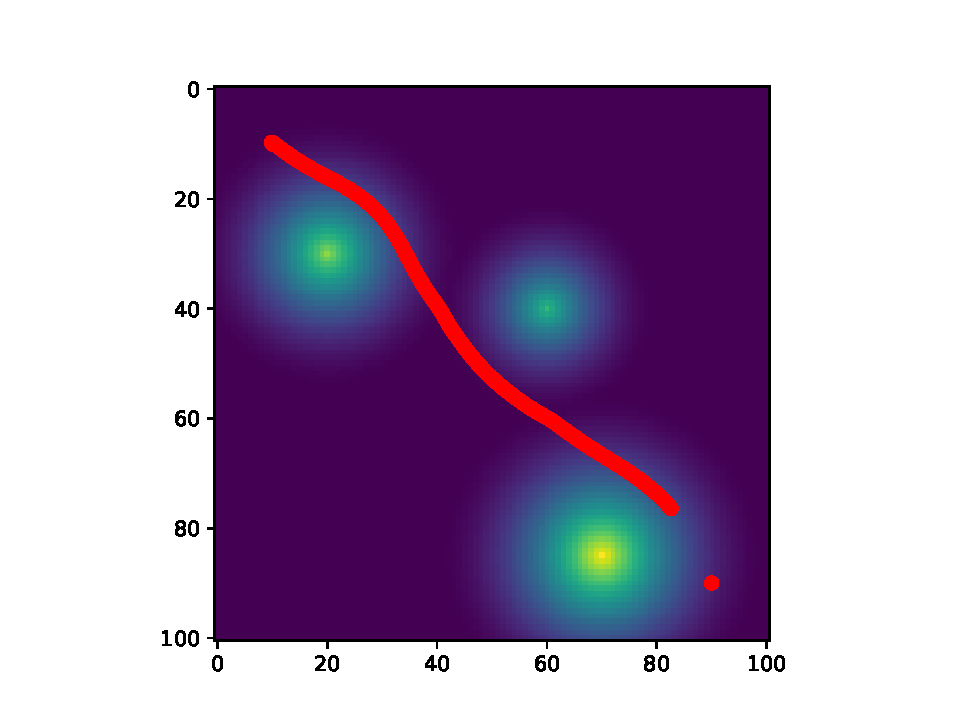
\includegraphics[width=.3\textwidth]{math/fig/hw4/ex6b/00100.pdf}
    }
    \subfigure[After 200 iters]{
    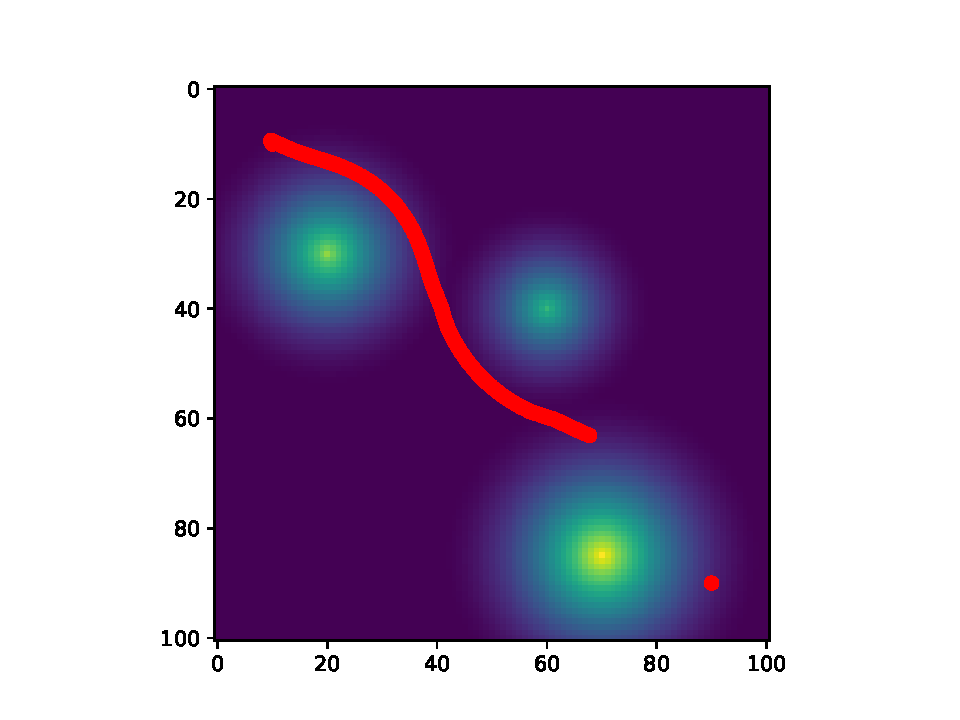
\includegraphics[width=.3\textwidth]{math/fig/hw4/ex6b/00200.pdf}
    }
    \subfigure[After 500 iters]{
    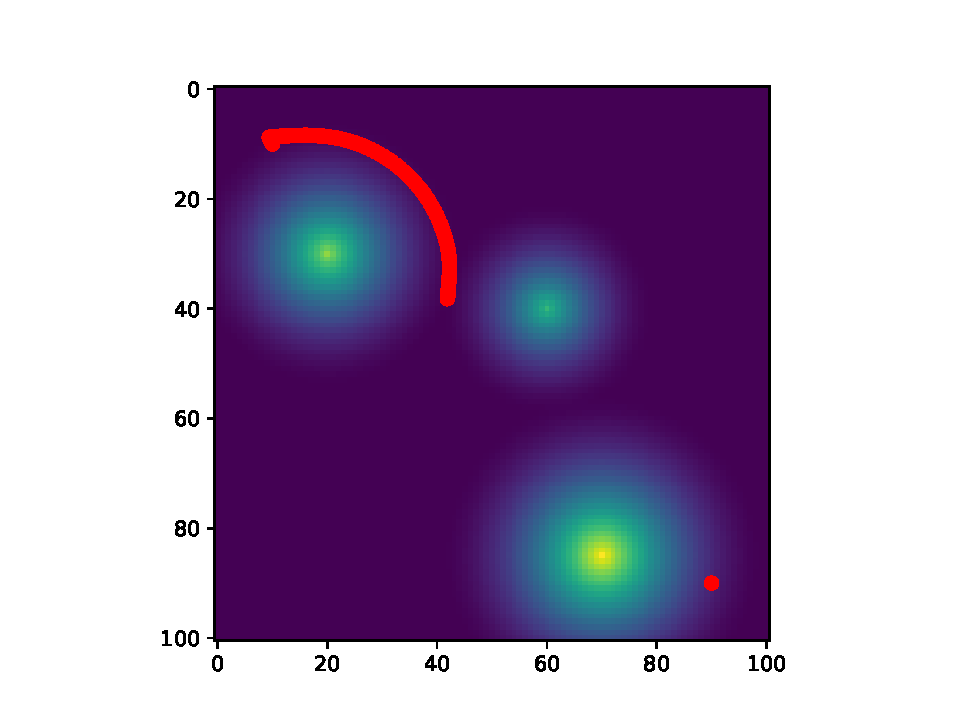
\includegraphics[width=.3\textwidth]{math/fig/hw4/ex6b/00500.pdf}
    }
    \caption{\textbf{Ex 6b}}
    \label{fig:hw4_ex6b}
\end{figure}

\subexercise
Figure \ref{fig:hw4_ex6c} is the result. The result is better because this algorithm considers the distance from not only the prior point but also the follow-up point.

\begin{figure}
    \centering
    \subfigure[After 100 iters]{
    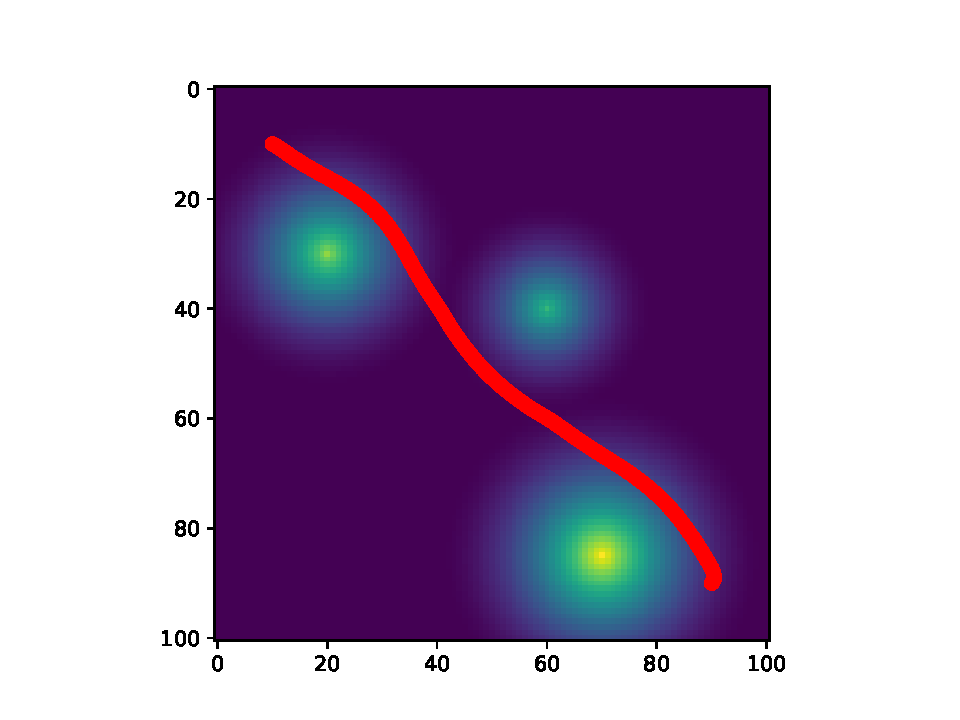
\includegraphics[width=.45\textwidth]{math/fig/hw4/ex6c/00100.pdf}
    }
    \subfigure[After 5000 iters]{
    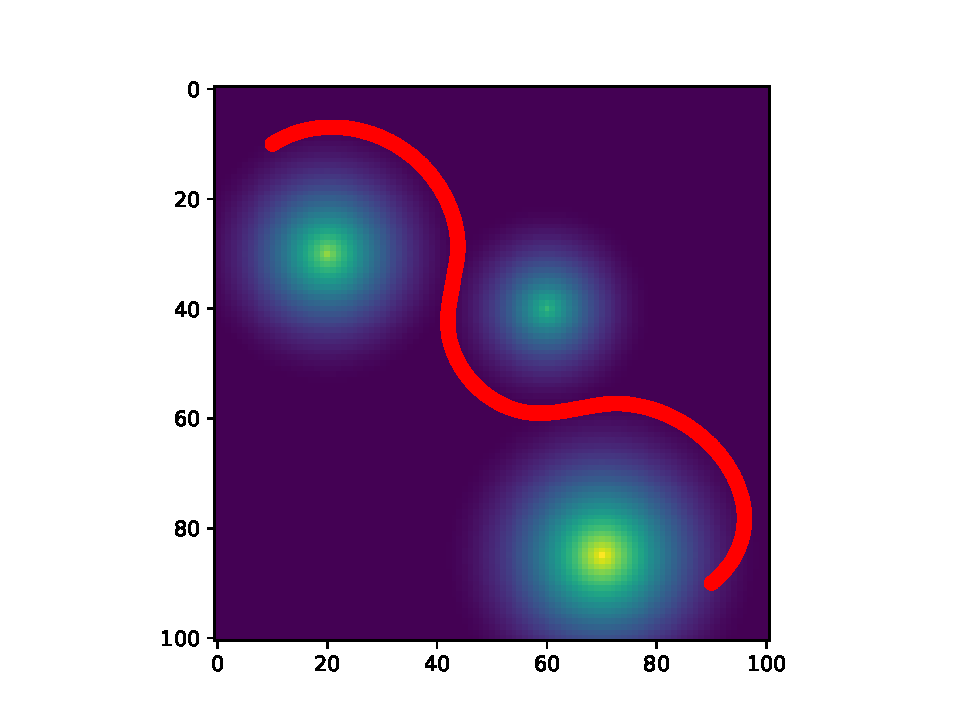
\includegraphics[width=.45\textwidth]{math/fig/hw4/ex6c/05000.pdf}
    }
    \caption{\textbf{Ex 6c}}
    \label{fig:hw4_ex6c}
\end{figure}

\subexercise
The final result would be different if the algorithm is initialized with different trajectories. Because the algorithm could only find the local minimum which is nearest to the initial trajectory. So the initialization matters a lot. See Figure \ref{fig:hw4_ex6d} for an example.

\begin{figure}
    \centering
    \subfigure[Initial Trajectory]{
    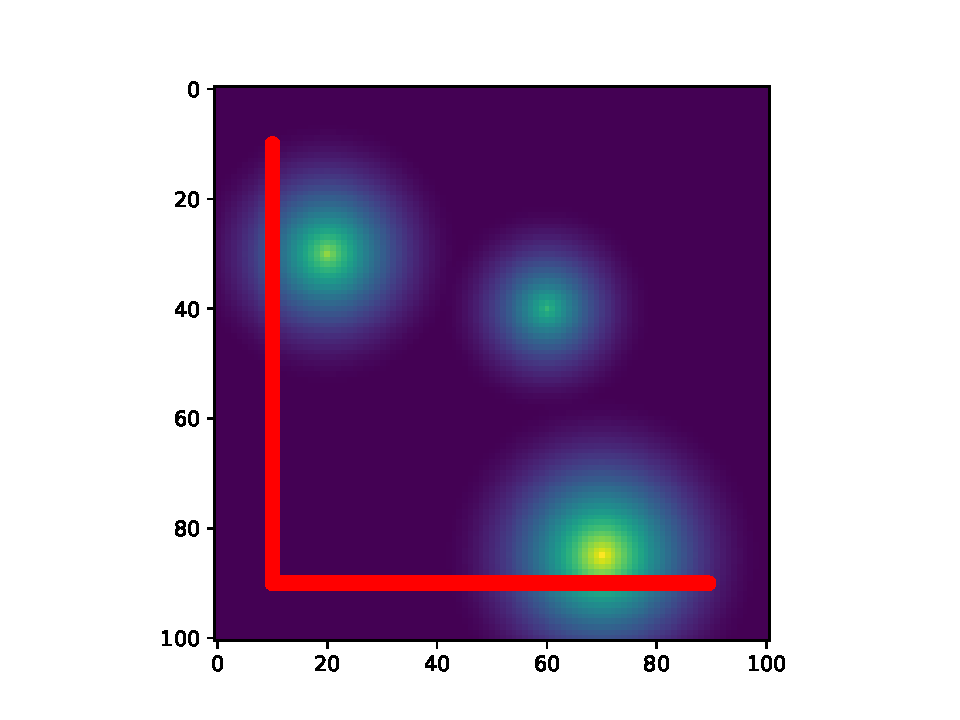
\includegraphics[width=.45\textwidth]{math/fig/hw4/ex6d/ex6d-init.pdf}
    }
    \subfigure[After 5000 iters]{
    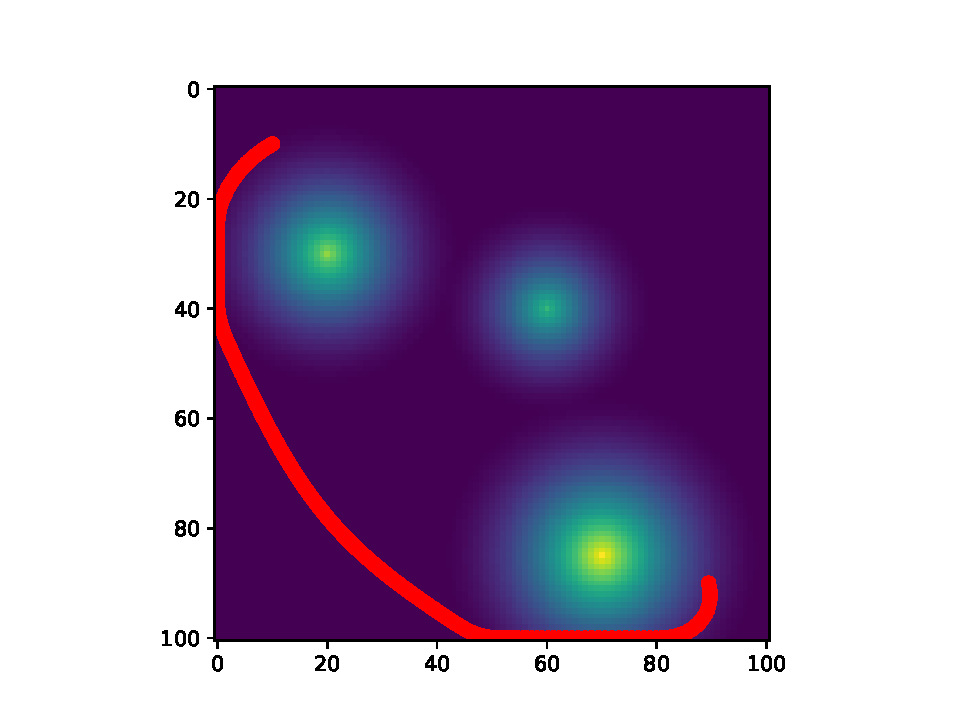
\includegraphics[width=.45\textwidth]{math/fig/hw4/ex6d/ex6d-final.pdf}
    }
    \caption{\textbf{Ex 6d}}
    \label{fig:hw4_ex6d}
\end{figure}

\subexercise
We can run the algorithm many times for different initial trajectories, and finally pick the best result.

\end{document}